% Compile with pdfLaTeX (also works with the default Overleaf compiler).
% Keep the image assets and horse-frames.pdf beside this file.
% The Motivation divider animates in desktop Acrobat Reader or Okular
% with JavaScript enabled; browser/Overleaf previews may show a still frame.
% Visual inspiration: https://www.instagram.com/p/DfXBRTqoBhW/
\documentclass[aspectratio=169,11pt]{beamer}
\usepackage[T1]{fontenc}
\usepackage[utf8]{inputenc}
\usepackage{mathpazo}
\usepackage{amsmath,amssymb}
\usepackage{tikz}
\usepackage{animate}
\usetikzlibrary{calc}
\usefonttheme{serif}
\usetikzlibrary{arrows.meta,positioning}
\newcommand{\cardC}{%
  \clubsuit\,\overline{\spadesuit}}
\newcommand{\cardS}{%
  \overline{\clubsuit}\,\spadesuit}
\newcommand{\cardB}{%
  \dot{\clubsuit}\,\dot{\spadesuit}}
% ---------- Editable palette ----------
\definecolor{Midnight}{HTML}{312744}
\definecolor{Violet}{HTML}{5E4B86}
\definecolor{BlueViolet}{HTML}{535F98}
\definecolor{Lilac}{HTML}{E6D9FA}
\definecolor{Sky}{HTML}{9DD5E3}
\definecolor{Rose}{HTML}{D77AAD}
\definecolor{Gold}{HTML}{C6AB6D}
\definecolor{Paper}{HTML}{F7F2EA}
\definecolor{WitchPurple}{HTML}{D0A6FF}

% ---------- Presentation information ----------
\title[The Dynamic Turn in Paraconsistency]{The Dynamic Turn in Paraconsistency}
\author{Rafael Ongaratto}
\date{}
\newcommand{\jointwork}{A joint work with Hans van Ditmarsch (IRIT/CNRS, Toulouse)}

\newcommand{\supervision}{Supervisor: Walter Carnielli (CLE, Campinas)}
\newcommand{\funding}{FAPESP Grant n\textordmasculine\ 2024/00807-6}
\hypersetup{pdftitle={The Dynamic Turn in Paraconsistency},
  pdfauthor={Rafael Ongaratto}}

% Four-point celestial ornament, drawn entirely in TikZ.
\newcommand{\sparkle}[4]{%
  \begin{scope}[shift={(#1,#2)},scale=#3]
    \fill[#4] (0,.34) .. controls (.035,.065) and (.065,.035) .. (.25,0)
      .. controls (.065,-.035) and (.035,-.065) .. (0,-.34)
      .. controls (-.035,-.065) and (-.065,-.035) .. (-.25,0)
      .. controls (-.065,.035) and (-.035,.065) .. (0,.34);
  \end{scope}}

% Coordinates below use a 16 x 9 canvas, matching the 16:9 slide.
\newcommand{\nightbackground}{%
  
\begin{tikzpicture}[remember picture,overlay]
  \begin{scope}[shift={(current page.south west)},x=1cm,y=1cm]
    \clip (0,0) rectangle (16,9);
    \shade[inner color=BlueViolet,outer color=Violet] (0,0) rectangle (16,9);
    % Fine, deterministic vector grain. Remove this loop for faster compiling.
    \pgfmathsetseed{731}
    \foreach \i in {1,...,1800}{%
      \pgfmathsetmacro{\grainx}{16*rnd}
      \pgfmathsetmacro{\grainy}{9*rnd}
      \pgfmathsetmacro{\grainsize}{.003+.009*rnd}
      \fill[Paper,opacity=.065] (\grainx,\grainy) circle[radius=\grainsize];}
    % Antique cloud linework, kept away from the text.
    \begin{scope}[draw=Sky,opacity=.24,line width=.45pt]
      \draw (-.5,7.25) .. controls (.1,7.8) and (.4,7.8) .. (.7,7.6)
        .. controls (.55,8.2) and (1.2,8.45) .. (1.5,8.05)
        .. controls (1.9,8.65) and (2.6,8.35) .. (2.55,7.95)
        .. controls (3.1,8.05) and (3.25,7.6) .. (3.5,7.65);
      \draw (-.3,7.1) .. controls (.3,7.5) and (.65,7.4) .. (.9,7.45)
        .. controls (1.1,8.05) and (1.65,7.9) .. (1.9,7.65)
        .. controls (2.3,7.95) and (2.8,7.7) .. (2.9,7.45);
      \draw (13.3,1.6) .. controls (13.5,2) and (13.9,2) .. (14.1,1.8)
        .. controls (14,2.35) and (14.7,2.6) .. (15,2.15)
        .. controls (15.5,2.7) and (16.1,2.35) .. (16.3,2.1);
      \draw (13.8,1.5) .. controls (14.1,1.9) and (14.5,1.9) .. (14.7,1.65)
        .. controls (15.2,2.1) and (15.6,1.8) .. (16.2,1.7);
    \end{scope}
    \sparkle{14.35}{7.65}{.8}{Lilac}
    \sparkle{14.98}{7.25}{.4}{Lilac}
    \sparkle{14.9}{8.15}{.25}{Lilac}
    \sparkle{1.05}{3.25}{.42}{Sky}
    \sparkle{.65}{1.15}{.5}{Gold}
    \sparkle{2.0}{.8}{.28}{Gold}
    \sparkle{14.65}{.8}{.62}{Gold}
    \sparkle{15.4}{1.4}{.3}{Gold}
    % Delicate eight-ray stars recall the poster's hand-drawn ornaments.
    \foreach \x/\y/\s in {1.25/1.7/.35,15.15/3.2/.26}{%
      \begin{scope}[shift={(\x,\y)},scale=\s,draw=Gold,opacity=.8,line width=.5pt]
        \draw (-1,0)--(1,0) (0,-1.35)--(0,1.35)
          (-.65,-.65)--(.65,.65) (-.65,.65)--(.65,-.65);
      \end{scope}}
  \end{scope}
  \end{tikzpicture}}

% ---------- Theme for subsequent content slides ----------
\setbeamertemplate{navigation symbols}{}
\setbeamercolor{normal text}{fg=Midnight,bg=Paper}
\setbeamercolor{structure}{fg=Violet}
\setbeamercolor{alerted text}{fg=Violet}
\setbeamercolor{frametitle}{fg=Violet}
\setbeamerfont{frametitle}{size=\LARGE,series=\mdseries}
\setbeamercolor{block title}{fg=Paper,bg=Violet}
\setbeamercolor{block body}{fg=Midnight,bg=Violet!8!Paper}
\setbeamercolor{section in head/foot}{fg=Lilac,bg=Midnight}
\setbeamercolor{toolbar}{fg=Lilac,bg=Midnight}
\setbeamercolor{section in toc}{fg=Violet}
\setbeamerfont{section in head/foot}{size=\scriptsize}
\setbeamerfont{section in toc}{size=\large}
\setbeamertemplate{section in head/foot shaded}[default][65]
\setbeamertemplate{section in toc}[sections numbered]
\setbeamersize{text margin left=1cm,text margin right=1cm}
% Clickable section toolbar, with a fine gold rule underneath.
\setbeamertemplate{headline}{%
  \begin{beamercolorbox}[wd=\paperwidth,ht=.48cm,dp=.17cm]{section in head/foot}
    \insertsectionnavigationhorizontal{\paperwidth}{\hskip.4cm}{\hskip.4cm}
  \end{beamercolorbox}%
  {\color{Gold}\hrule height .45pt}}
\setbeamertemplate{frametitle}{\vspace{.3cm}\insertframetitle\par
  \vspace{.1cm}{\color{Gold}\rule{\textwidth}{.35pt}}}
% Bottom toolbar: author, talk title, summary/back/next links, slide number.
\setbeamertemplate{footline}{%
  {\color{Gold}\hrule height .45pt}%
  \begin{beamercolorbox}[wd=\paperwidth,ht=.4cm,dp=.18cm,leftskip=.5cm,rightskip=.5cm]{toolbar}
    \usebeamerfont{footline}\insertshortauthor\hfill
    \insertshorttitle\hfill
    \hyperlink{summary}{Summary}\hspace{.28cm}
    \hyperlinkslideprev{\ensuremath{\lhd}}\hspace{.18cm}
    \hyperlinkslidenext{\ensuremath{\rhd}}\hspace{.28cm}
    \insertframenumber\,/\,\inserttotalframenumber
  \end{beamercolorbox}}
\setbeamerfont{footline}{size=\fontsize{6.5}{8}\selectfont}
\setbeamertemplate{itemize item}{\color{Violet}\small$\diamond$}
\setbeamertemplate{itemize subitem}{\color{Violet}\tiny$\diamond$}

% Section divider pages also serve as editable starting points for the talk.
\newcommand{\sectiondivider}[1][Violet]{%
  \begin{frame}[c]
    \centering
    {\color{Rose}\large\thesection\par}
    \vspace{.35cm}
    {\color{#1}\LARGE\insertsectionhead\par}
    \vspace{.4cm}
    {\color{Gold}\rule{3cm}{.5pt}\par}
  \end{frame}}

% Actual motion: all 15 pages of horse-frames.pdf play at 10 fps.
% method=ocg lets the heading and violet veil appear above the animation.
% Source and playback instructions: HORSE-ANIMATION.md.
\newcommand{\horsemotionbackground}{%
  \begin{tikzpicture}[remember picture,overlay]
    \fill[Midnight] (current page.south west)
      rectangle (current page.north east);
    \node[inner sep=0pt] at (current page.center) {%
      \animategraphics[method=ocg,autoplay,loop,nomouse,poster=first,
        width=\paperwidth,height=\paperheight,keepaspectratio]
        {10}{horse-frames}{}{}%
    };
    \fill[Midnight,opacity=.65] (current page.south west)
      rectangle (current page.north east);
  \end{tikzpicture}%
}

% Custom title page: all lettering remains editable and selectable.
\setbeamertemplate{title page}{%
  \nightbackground
  \begin{tikzpicture}[remember picture,overlay]
  \begin{scope}[shift={(current page.south west)},x=1cm,y=1cm]
    \node[text=Sky,font=\fontsize{29}{33}\selectfont,inner sep=0]
      at (8,7.45) {The Dynamic Turn};
    \node[text=Lilac,font=\fontsize{29}{33}\selectfont\itshape,inner sep=0]
      at (8,6.4) {in Paraconsistency};
    \draw[Rose,line width=.7pt] (6.9,5.7)--(7.82,5.7)
      (8.18,5.7)--(9.1,5.7);
    \sparkle{8}{5.7}{.22}{Rose}
    \node[text=Paper,font=\fontsize{17}{21}\selectfont]
      at (8,5.12) {\insertauthor};
    \node[text=Lilac,font=\fontsize{10.5}{14}\selectfont]
      at (8,4.48) {\jointwork};
    \node[text=Lilac,font=\fontsize{10}{13}\selectfont]
      at (8,2.55) {\supervision};
    \node[text=Paper,font=\fontsize{9}{12}\selectfont]
      at (8,2.02) {\funding};
    % Pale purple lettering stays legible on the violet background.
    % A subtle offset shadow and italic capitals give the event a wordmark.
    \node[text=Midnight,opacity=.45,font=\fontsize{28}{32}\selectfont\itshape]
      at (8.025,.82) {{\fontsize{19}{23}\selectfont\upshape IV}\ WITCH};
    \node[text=WitchPurple,font=\fontsize{28}{32}\selectfont\itshape]
      at (8,.85) {{\fontsize{19}{23}\selectfont\upshape IV}\ WITCH};
    \sparkle{5.4}{.85}{.34}{WitchPurple}
    \sparkle{10.6}{.85}{.34}{WitchPurple}
  \end{scope}
  \end{tikzpicture}}

\begin{document}

\begin{frame}[plain,noframenumbering]
  \titlepage
\end{frame}

\begin{frame}[label=summary]{Summary}
  \vspace{.25cm}
  \tableofcontents[hideallsubsections]
\end{frame}

% Suggested outline: edit these section names to match your talk.
% The Summary and top toolbar update automatically after two compilations.
% Insert your content frames after each divider.
\section[Motivation]{Motivation}
\begingroup
  \setbeamertemplate{background canvas}{\horsemotionbackground}
  \sectiondivider[Paper]
\endgroup

\begin{frame}{Contradictions?}
    In the literature, two main types of interpretations of contradictions are distinguished:
\begin{columns}
    \begin{column}{0.48\textwidth}
        \begin{block}{Epistemic contradiction}
        \begin{itemize}
            \item Inconsistencies in empirical theories
            \item Failure of measuring instruments
            \item Temporary contradictions
        \end{itemize}
        \end{block}
    \end{column}

    \begin{column}{0.48\textwidth}
        \begin{block}{\textit{Dialetheia}}
\begin{itemize}
\item Ontological contradictions
\item Example: Liar Paradox
\item Static Contradictions
\end{itemize}
        \end{block}
    \end{column}

\end{columns}

\end{frame}


\begin{frame}{\textit{Para}consistency: beyond consistency, beside consistency?}
   \small Usually, the difference in these approaches is characterized by the type of logic adopted by each logician. 
    \begin{columns}
    \begin{column}{0.48\textwidth}
        \begin{block}{\textit{Epistemic}-reasoner}
        \begin{itemize}
           \item Adopts more expressive logics.
           \item Classical reasoning is available at hand.
           \item Translation of classical logic into some fragment of the adopted logic.
        \end{itemize}
        \end{block}
    \end{column}

    \begin{column}{0.48\textwidth}
        \begin{block}{\textit{Dialetheic}-reasoner}
\begin{itemize}
\item Adopts less expressive logics
\item Classical reasoning is not available at hand.
\item Classical logic is not a fragment of the adopted logic.
\end{itemize}
        \end{block}
    \end{column}

\end{columns}
\end{frame}

\begin{frame}{Take your pick, LP or LFI1?}
Consider $P$ to be a denumerable set of propositional variables. Then, the language of LP, $\mathcal{L}_{LP}$ is defined as
    \[\alpha := p \mid \neg\alpha \mid \alpha \land \alpha \]
The language of LFI1, $\mathcal{L}_{LFI1}$, is defined as 
\[\alpha := p \mid \neg\alpha \mid \alpha \land \alpha \mid \circ\alpha\]
\end{frame}


\begin{frame}{Take your pick, LP or LFI1?}
\centering
\vspace{-.6cm}
\renewcommand{\arraystretch}{1.35}
\setlength{\arraycolsep}{6pt}

% Binary connectives
\[
\begin{array}{|c|ccc|}
\hline
\land & 1 & \tfrac12 & 0 \\ \hline
1        & 1        & \tfrac12 & 0 \\
\tfrac12 & \tfrac12 & \tfrac12 & 0 \\
0        & 0        & 0        & 0 \\ \hline
\end{array}
\qquad
\begin{array}{|c|ccc|}
\hline
\lor & 1 & \tfrac12 & 0 \\ \hline
1        & 1 & 1        & 1        \\
\tfrac12 & 1 & \tfrac12 & \tfrac12 \\
0        & 1 & \tfrac12 & 0        \\ \hline
\end{array}
\qquad
\begin{array}{|c|ccc|}
\hline
\to & 1 & \tfrac12 & 0 \\ \hline
1        & 1 & \tfrac12 & 0 \\
\tfrac12 & 1 & \tfrac12 & 0 \\
0        & 1 & 1        & 1 \\ \hline
\end{array}
\]

\medskip

% Unary connectives
\[
\begin{array}{|c|cccc|}
\hline
x & \neg x & \circ x & \bullet x & \sim x \\ \hline
1        & 0        & 1 & 0 & 0 \\
\tfrac12 & \tfrac12 & 0 & 1 & 0 \\
0        & 1        & 1 & 0 & 1 \\ \hline
\end{array}
\]

\medskip
{\small
$\sim\alpha := \neg\alpha\land\circ\alpha$,
\qquad
$\alpha\to\beta := \sim\alpha\lor\beta$.
}

\end{frame}


\begin{frame}{Limitations}
    LP is a proper fragment of LFI1. We know that LFI1 is not a proper logic to deal with \textit{dialetheias} of the type of semantic paradoxes, as
    \[QLFI1 + \text{self-reference} + \text{T-schema} \Rightarrow \text{Trivialization}\]
    However, is it enough to represent epistemic contradictions?

    
\centering
    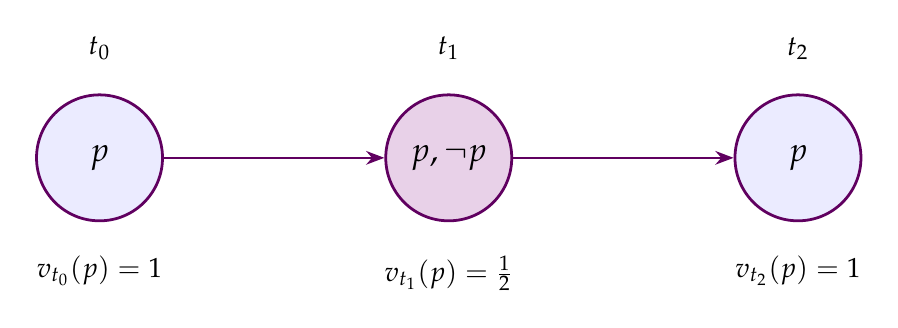
\begin{tikzpicture}[
    >=Stealth,
    state/.style={
        circle,
        draw=violet!75!black,
        line width=1pt,
        minimum size=1.6cm,
        align=center,
        font=\large
    },
    transition/.style={
        ->,
        thick,
        draw=violet!75!black
    },
    node distance=2.8cm
]

\node[state,fill=blue!8] (t0) {$p$};
\node[state,fill=violet!18,right=of t0] (t1) {$p,\neg p$};
\node[state,fill=blue!8,right=of t1] (t2) {$p$};

\draw[transition] (t0) -- (t1);
\draw[transition] (t1) -- (t2);

\node[above=0.3cm of t0] {$t_0$};
\node[above=0.3cm of t1] {$t_1$};
\node[above=0.3cm of t2] {$t_2$};

\node[below=0.3cm of t0] {$v_{t_0}(p)=1$};
\node[below=0.3cm of t1] {$v_{t_1}(p)=\tfrac12$};
\node[below=0.3cm of t2] {$v_{t_2}(p)=1$};

\end{tikzpicture}
\end{frame}

\begin{frame}{Static Contradictions}
    LFI1 is a three-valued logic. Each valuation represents a ``state of the world'' at a given moment. There is no tool to represent change from one state to another \textit{within} this logic.\\~\\
    Contradictions in LFI1 are still \textbf{static}. To properly formalize epistemic contradictions, we need a \textbf{dynamic} picture.

    
\end{frame}

\section[Paraconsistent Epistemic Logic]{Paraconsistent epistemic logic}
\sectiondivider

\begin{frame}
The first step towards making LFI1 epistemic is adding agents and knowledge operators. Consider the multi-modal language of KLFI1, $\mathcal{L}_\Box$, for a set $I$ of agents of finite cardinality such that $i \in I$, 
\[\alpha := p \mid \neg\alpha \mid \alpha \land \alpha \mid \Box_i\alpha\]

Let us consider KLFI1, the minimal normal modal logic based on LFI1.
\end{frame}

\begin{frame}{KLFI1}
A KLFI1-relational model is a triple $\mathcal{M} = \langle W, \{R_i\}_{i \in I}, v\rangle$, where 
\\$W \neq \emptyset$, \\$R_i \subseteq W \times W$, \\$v$ is an LFI1-valuation that adds the following condition for the box modality and its dual:

\[v(\Box_i\alpha, w) = \inf\{v(\alpha, w'): wR_iw'\}\]
\[v(\Diamond_i\alpha, w) = \sup\{v(\alpha, w'): wR_iw'\}\]

LFI1-relational frames are defined as $\mathcal{F} = \langle W, \{R_i\}_{i\in I}\rangle$, where $\mathcal{M} = \langle W, \{R_i\}_{i \in I}, v\rangle$ is an LFI1-relational model over $\mathcal{F}$.
\end{frame}

\begin{frame}{KLFI1}
    KLFI1 is characterized by the class of arbitrary LFI1-relational frames.
    \\~\\
    KLFI1 is axiomatized by extending LFI1 with the following axioms and rules, where $\Diamond_i\alpha$ is an abbreviation for $\neg\Box_i\neg\alpha$:

    \[\begin{array}{ll}
    (K) & \Box_i(\alpha \rightarrow \beta) \rightarrow (\Box_i \alpha \rightarrow \Box_i\beta) \\ 
        (K1) &  \Box_i(\alpha \rightarrow \beta) \rightarrow (\Diamond_i\alpha \rightarrow \Diamond_i \beta)\\
         (K2) & \Diamond_i(\alpha \lor \beta) \rightarrow \Diamond_i \alpha \lor \Diamond_i\beta\\
(K3) & (\Diamond_i\alpha \rightarrow \Box_i\beta) \rightarrow (\Box_i(\alpha \rightarrow \beta))\\
(Nec) & \vdash \alpha \Rightarrow\ \vdash \Box_i\alpha\\
    \end{array}\]

    S5LFI1, the standard logic of knowledge, is characterized by the reflexive, transitive and euclidean class of LFI1-relational frames.
\end{frame}

\begin{frame}{S5LFI1}
\vspace{-1.1cm}
\small\begin{columns}[T,onlytextwidth]

  \begin{column}{0.48\textwidth}
    \begin{block}{Epistemic axioms}
      \begin{itemize}
        \setlength{\itemsep}{0.8ex}

        \item[\(\mathbf{T}_i\)] \textbf{Truth}\\
          \(\Box_i\alpha \supset \alpha\)

        \item[\(\mathbf{D}_i\)] \textbf{Consistency}\\
          \(\Box_i\alpha \rightarrow \Diamond_i\alpha\)

        \item[\(\mathbf{4}_i\)] \textbf{Positive introspection}\\
          \(\Box_i\alpha \rightarrow \Box_i \Box_i\alpha\)

        \item[\(\mathbf{5}_i\)] \textbf{Negative introspection}\\
          \(\neg \Box_i\alpha \rightarrow \Box_i\neg \Box_i\alpha\)
      \end{itemize}
    \end{block}
  \end{column}

  \begin{column}{0.48\textwidth}
    \begin{block}{Dual instances}
      \begin{itemize}
        \setlength{\itemsep}{0.8ex}

        \item[\(\mathbf{T}'_i\)] \textbf{Dual truth}\\
          \(\alpha \rightarrow \Diamond_i\alpha\)

       
          

        \item[\(\mathbf{4}'_i\)] \textbf{Dual positive introspection}\\
          \(\Diamond_i\Diamond_i\alpha \rightarrow \Diamond_i\alpha\)

        \item[\(\mathbf{5}'_i\)] \textbf{Dual negative introspection}\\
          \(\Diamond_i\Box_i\alpha \rightarrow \Box_i\alpha\)
      \end{itemize}
    \end{block}
  \end{column}

\end{columns}

*($D_i$) is self-dual
\end{frame}

\begin{frame}
\centering

\includegraphics[width=\textwidth,height=0.8\textheight,keepaspectratio]{Dois olhares sob a luz do lampião.png}

Anne wants to know which card is facing the table, and she relies on her friend's information, which is not always truthful nor consistent. 
\end{frame}
% Preamble:
% \usepackage{tikz}
% \usetikzlibrary{arrows.meta}

\begin{frame}{Anne's card}
\centering

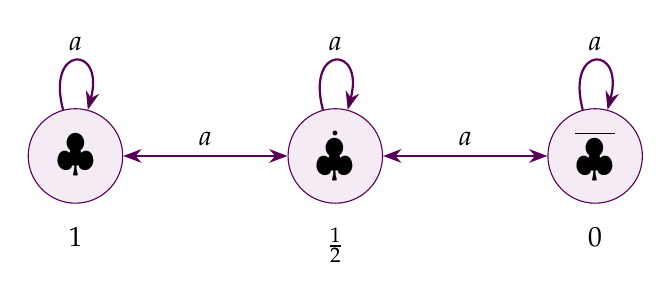
\begin{tikzpicture}[
    >=Stealth,
    world/.style={
        circle,
        draw=violet!70!black,
        fill=violet!8,
        minimum size=1.2cm,
        font=\LARGE
    },
    relation/.style={
        draw=violet!70!black,
        thick
    },
    every loop/.style={looseness=7}
]

% Three possible information states
\node[world] (T) at (0,0)   {$\clubsuit$};
\node[world] (B) at (3.3,0) {$\dot{\clubsuit}$};
\node[world] (F) at (6.6,0) {$\overline{\clubsuit}$};

% Universal accessibility
\draw[relation,<->]
    (T) -- node[above] {$a$} (B);
\draw[relation,<->]
    (B) -- node[above] {$a$} (F);

% Reflexive arrows at every world
\foreach \w in {T,B,F}{
    \draw[relation,->]
        (\w) edge[loop above] node[above] {$a$} (\w);
}

% Truth values
\node[below=5pt] at (T.south) {$1$};
\node[below=5pt] at (B.south) {$\tfrac12$};
\node[below=5pt] at (F.south) {$0$};

\end{tikzpicture}

\medskip
{\small
$\clubsuit$: clubs
\qquad
$\dot{\clubsuit}$: contradictory information
\qquad
$\overline{\clubsuit}$: not clubs
}

\medskip
Anne has received no information distinguishing these worlds.

\end{frame}

\section[Action Models]{Action Models}
\sectiondivider

\begin{frame}{Learning Information}
    Learning new information requires making transformations in Kripke models. With the tools of Dynamic Epistemic Logic (DEL), it is possible to do so.

    Consider a countably infinite index set $E$ representing an enumeration of actions such that $e \in E$, and a finite set $A$ of agents such that $a \in A$. The language of action models over LFI1, $\mathcal{L}_{AM}$, is defined as,
    
    \[\alpha := p \mid \neg\alpha \mid \circ\alpha \mid \alpha \land \alpha \mid \Box_i\alpha \mid [e]\alpha\]
\end{frame}

\begin{frame}{Action Models}
An S5LFI1 {\em action model} $U$ is a structure $\langle \mathit{E}, \{\sim_i\}_{i\in N}, \mathrm{pre}\rangle$, such that $E$ is a set of \emph{actions}, $\sim_i$ is an equivalence relation for an agent $i$, and {\em precondition function} $\mathrm{pre}:\mathit{E} \mapsto \mathcal{L}_{AM}$ assigns a formula to each action. The formula $\mathrm{pre}(e)$ is the \emph{precondition} for the execution of the action $e$.
\end{frame}
\begin{frame}
    \begin{block}{AMLFI1}
   The logic AMLFI1 is characterized over the language $\mathcal{L}_{AM}$ by the axioms and rules of S5LFI1 plus the following axioms and rules:
\[
\begin{array}{l@{\qquad}l}
AM1 & [U,e]p \equiv (\text{pre}(e) \rightarrow p)\\
AM2 & [U,e]\neg\alpha \equiv (\text{pre}(e) \rightarrow \neg[U,e]\alpha)\\
AM3 & [U,e]\bullet\alpha \equiv (\text{pre}(e) \rightarrow \bullet[U,e]\alpha)
\\
AM4 & [U,e](\alpha \land \beta)
      \equiv ([U,e]\alpha \land [U,e]\beta)\\
AM5 & [U,e]K_i\alpha
      \equiv (\text{pre}(e) \rightarrow \bigwedge_{e \sim_i f} K_i[U,f]\alpha)\\
RE  & \vdash\theta \equiv \gamma \Rightarrow\ \vdash\alpha \equiv \alpha(\theta/\gamma)
\end{array}
\]
\end{block}
We recall that $\equiv$ is strong equivalence, definable in LFI1 as $(\alpha \leftrightarrow \beta) \land (\neg\alpha \leftrightarrow \neg\beta)$.
\end{frame}
\section[Update Models]{Update Models}
\sectiondivider

\section{Friendly Contradictions}
\sectiondivider

% Example content frame (copy into the relevant section above):
% \begin{frame}{A dynamic perspective}
%   Your text and formulas go here.
%   \begin{block}{Definition}
%     Insert the exact definition used in your work.
%   \end{block}
% \end{frame}

\end{document}
